\chapter{\bf{Use Cases}}

\noindent Per poter rappresentare le user stories sopra descritte, utilizziamo gli Use Case Diagrams, dei diagrammi che rappresentano le interazioni tra gli utenti e il sistema.
In questo scenario, l'attore principale è l'utente che  interagisce con il sistema del cancello automatico attraverso i pulsanti B1, B2 e B3.


\section{Apertura Cancello [US1-US10-US14]}
L'utente ha la possibilità, in prossimità del cancello, di richiederne l'apertura premendo il pulsante B1. Quando il sistema rileva che il pulsante B1 è stato premuto e il cancello è nelle condizioni specificate (chiuso o in chiusura), avvia il processo di apertura del cancello. Il dispositivo inoltre fornisce un feedback visivo ottenuto dall'attivazione di un segnale luminoso, identificato dal lampeggiare di un LED giallo con una frequenza 0.5 Hz.
Il dispositivo, inoltre, permette di verificare la completa apertura del cancello tramite l'accensione di tutti i LED: giallo, rosso e verde (figura \ref{usecase1}).

\begin{figure}[H]
    \centering
    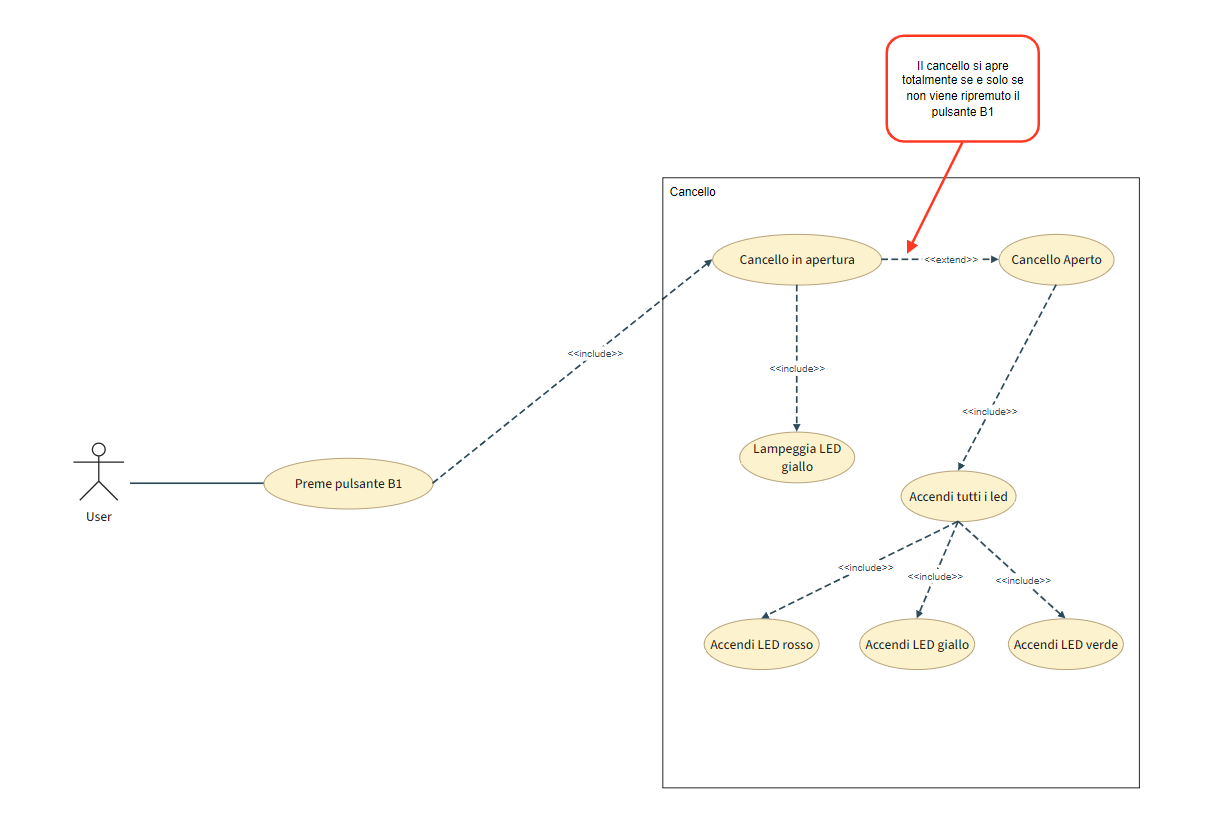
\includegraphics[width=0.9\textwidth]{figures/usecase_1.png}
    \caption{Apertura Cancello}
    \label{usecase1}
\end{figure}


\section{Chiusura Cancello [US2-US10-US13]}
L'utente ha la possibilità, in prossimità del cancello, di richiederne la chiusura premendo il pulsante B1. Quando il sistema rileva che il pulsante B1 è stato premuto e il cancello è nelle condizioni specificate (aperto o in apertura), avvia il processo di chiusura del cancello. Il dispositivo inoltre fornisce un feedback visivo ottenuto dall'attivazione di un segnale luminoso, identificato dal lampeggiare di un LED giallo con una frequenza 0.5 Hz.
Il dispositivo, inoltre, permette di verificare la completa chiusura del cancello tramite lo spegnimento di tutti i LED (figura \ref{usecase2}).

\begin{figure}[H]
    \centering
    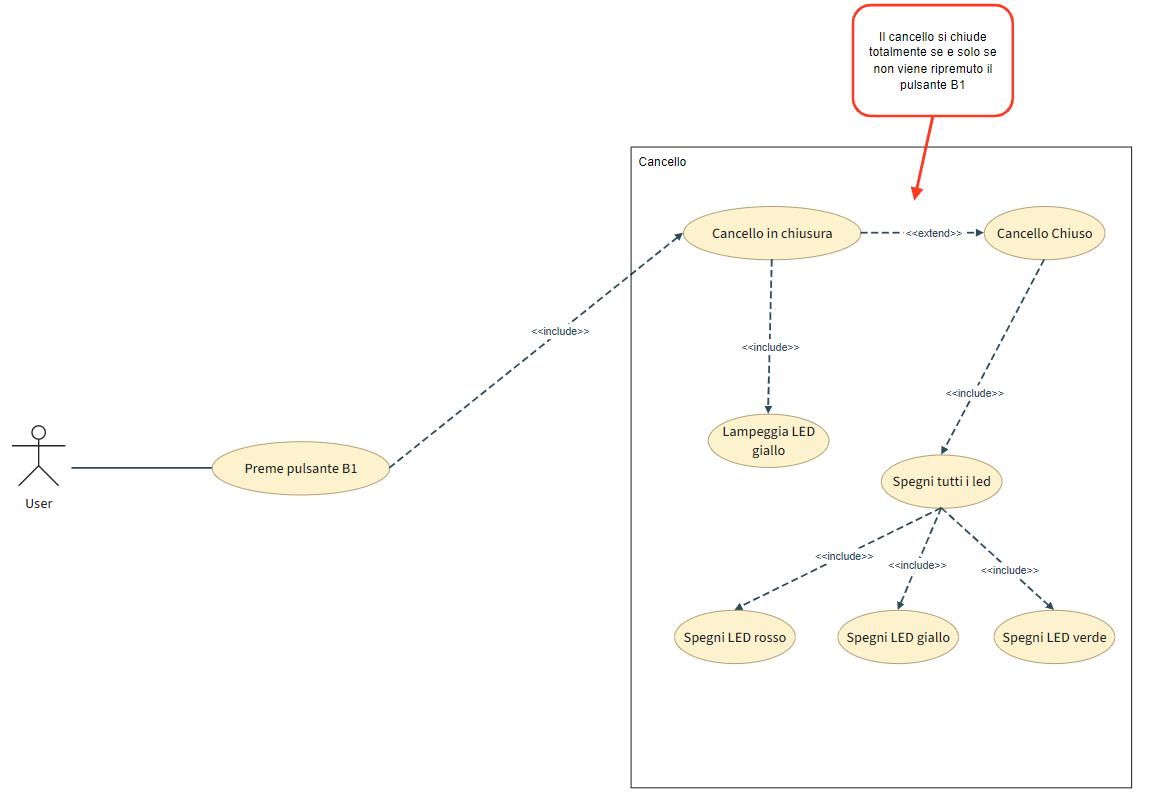
\includegraphics[width=0.9\textwidth]{figures/usecase_2.png}
    \caption{Chiusura Cancello}
    \label{usecase2}
\end{figure}


\section{Regolazione Tempo di Chiusura Automatica [US3]}
L'utente ha la possibilità di regolare il tempo di chiusura automatica del cancello andando a determinare quanto esso debba rimanere aperto prima di chiudersi automaticamente.
Quando il cancello è chiuso, l'utente preme il pulsante B2 per effettuare la regolazione. Se il tempo di chiusura automatica è inferiore a 120 secondi, ogni pressione del pulsante B2 aumenta il tempo di 10 secondi. Se il tempo è già a 120 secondi, premendo nuovamente B2 il tempo viene riportato a 10 secondi (figura \ref{usecase3}).


\section{Regolazione Tempo di Lavoro [US4]}
L'utente ha la possibilità  di richiedere la regolazione della durata della fasi di apertura e chiusura del cancello premendo l'apposito pulsante (B3) solo quando il cancello è chiuso. Questa azione è essenziale per impostare la durata delle due fasi del cancello. Ogni pressione del pulsante incrementa la durata di 10 secondi e, se il tempo di lavoro è al suo massimo (120 secondi), esso ritorna a 10 secondi (figura \ref{usecase3}).

\begin{figure}[H]
    \centering
    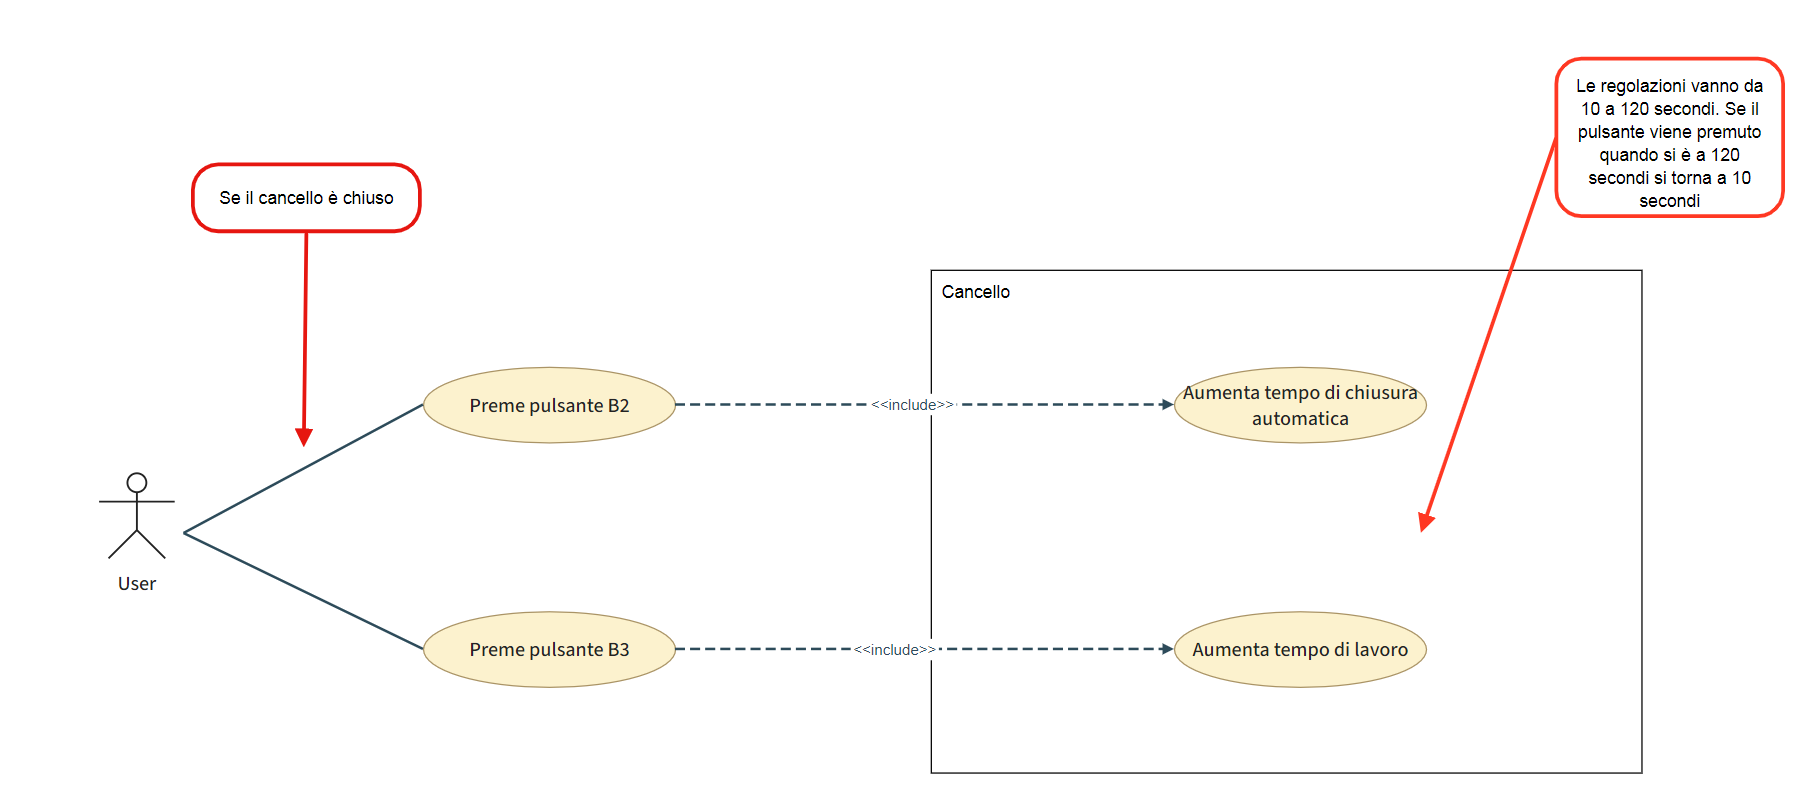
\includegraphics[width=0.9\textwidth]{figures/usecase_3.png}
    \caption{Regolazioni}
    \label{usecase3}
\end{figure}


\section{Riapertura Automatica con Rilevazione Ostacolo [US5-US14]}
Il dispositivo, in caso di rilevamento, tramite il sensore di presenza (P1), di un ostacolo durante la fase di chiusura, può effettuare la riapertura automatica del cancello.
Questa azione è essenziale per evitare danni al cancello e garantire la sicurezza delle persone e degli oggetti presenti. 
Il dispositivo fornisce un feedback in caso di apertura completa del cancello, dato dall'accensione di tutti i LED (figura \ref{usecase5}).


\section{Gestione Richieste in Presenza di Ostacoli [US6-US12]}
Il dispositivo, nel caso in cui il sensore di presenza (P1) sia attivo, ignora le richieste di apertura o chiusura del cancello.
Questa azione è essenziale per prevenire movimenti non sicuri del cancello in presenza di ostacoli o persone.
Il dispositivo fornisce un feedback visivo in caso di presenza di un ostacolo, dato dal lampeggio del LED verde con frequenza di 1 Hz per un tempo di 30 secondi o finché l'ostacolo non viene più rilevato (figura \ref{usecase5}).

\begin{figure}[H]
    \centering
    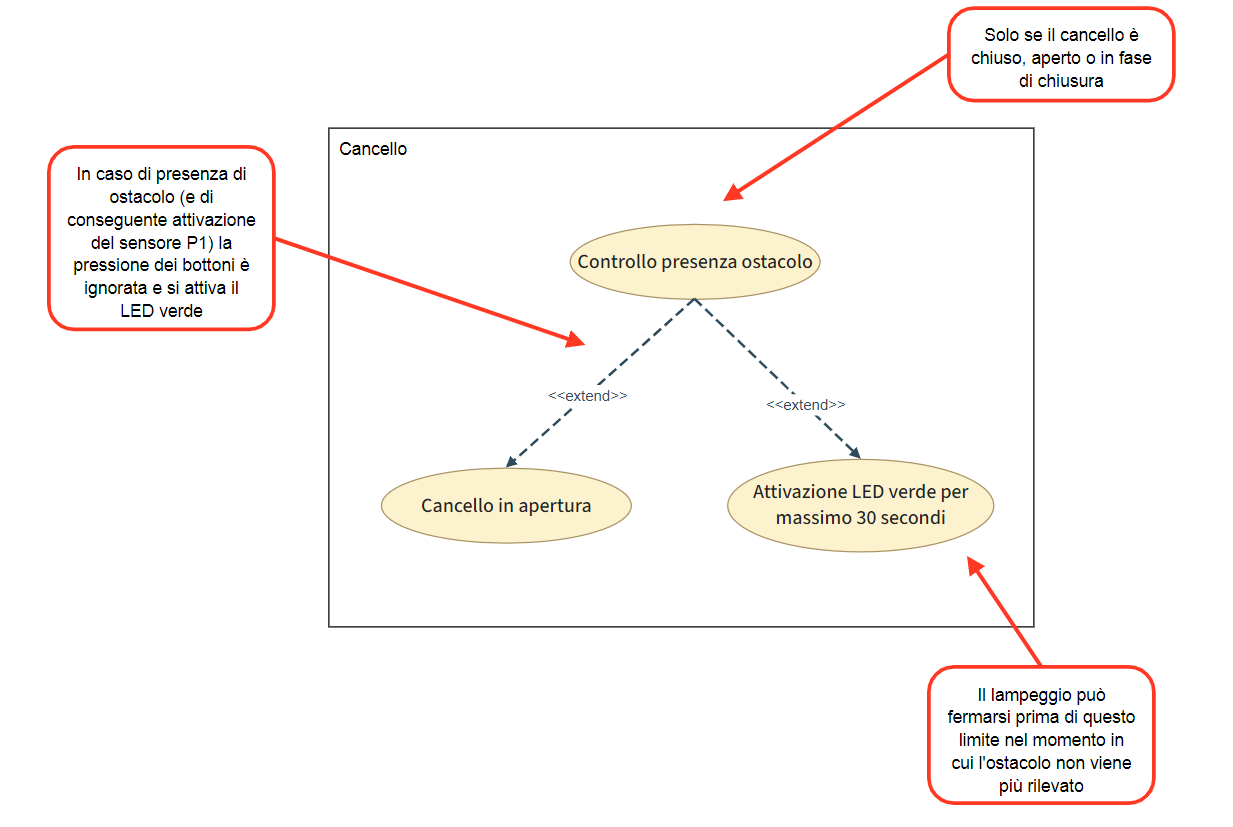
\includegraphics[width=0.9\textwidth]{figures/usecase_5.png}
    \caption{Controllo Ostacolo e Gestione Richieste}
    \label{usecase5}
\end{figure}


\section{Determinazione e Comunicazione Stato Cancello [US7-US13]}
Il dispositivo, tramite il sensore di presenza (P2), decreta lo stato di chiusura completa del cancello.
Questa azione è essenziale per determinare correttamente lo stato del cancello che si considera chiuso quando il sensore è attivo (figura \ref{usecase7}). 
Il dispositivo fornisce un feedback visivo in caso il cancello risulti completamente chiuso, dato dallo spegnimento di tutti i LED.

\begin{figure}[H]
    \centering
    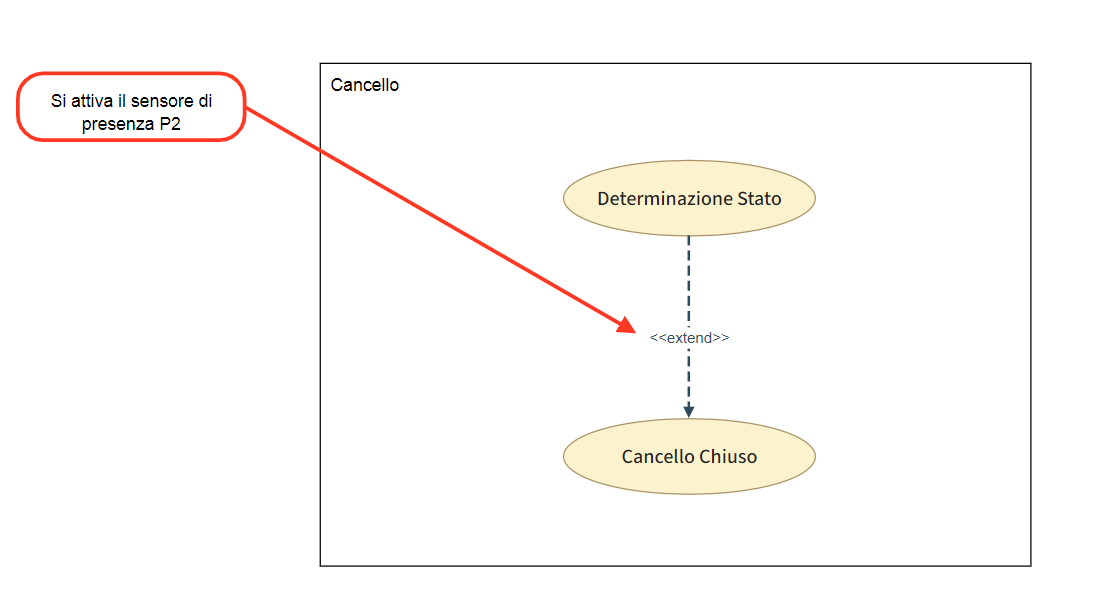
\includegraphics[width=0.9\textwidth]{figures/usecase_7.png}
    \caption{Determinazione Stato}
    \label{usecase7}
\end{figure}


\section{Gestione dello Stato di Errore [US8-US11]}
Il dispositivo entra in uno stato di errore nel caso in cui il sensore di presenza (P2) non si attivi dopo il tempo di lavoro previsto durante la fase di chiusura del cancello.
Questa azione è essenziale per far sì che l'utente venga avvisato in caso di malfunzionamento del sensore.
Il dispositivo fornisce un feedback visivo dello stato di errore, dato dall'accensione del LED rosso nel caso in cui il cancello non si chiuda entro 10 secondi dal completamento del tempo di lavoro (figura \ref{usecase8}).

\begin{figure}[H]
    \centering
    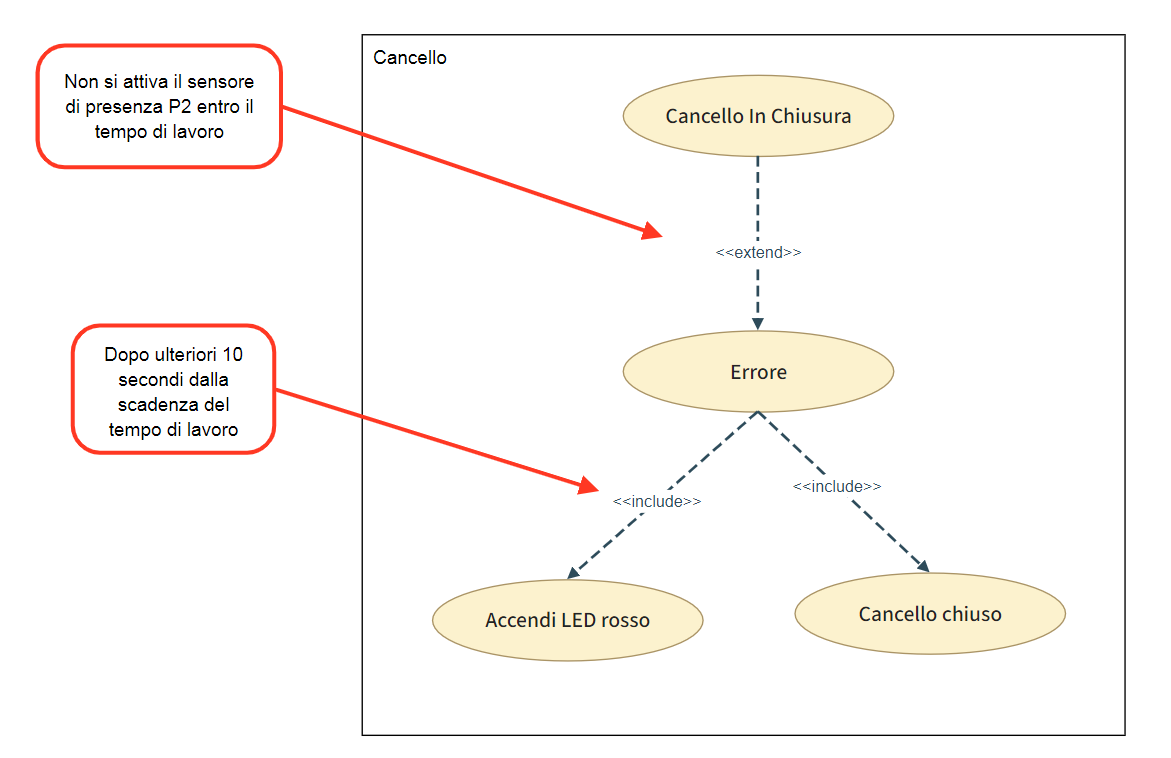
\includegraphics[width=0.9\textwidth]{figures/usecase_8.png}
    \caption{Stato di Errore}
    \label{usecase8}
\end{figure}


\section{Chiusura automatica all'accensione [US9]}
L'utente ha la possibilità di richiedere che il dispositivo avvii la procedura di chiusura del cancello automatico quando il dispositivo viene acceso per la prima volta, solo se i due sensori di presenza P1 e P2 non sono attivi.
Questa azione è essenziale per garantire la corretta chiusura del cancello all'accensione del dispositivo.

\begin{figure}[H]
    \centering
    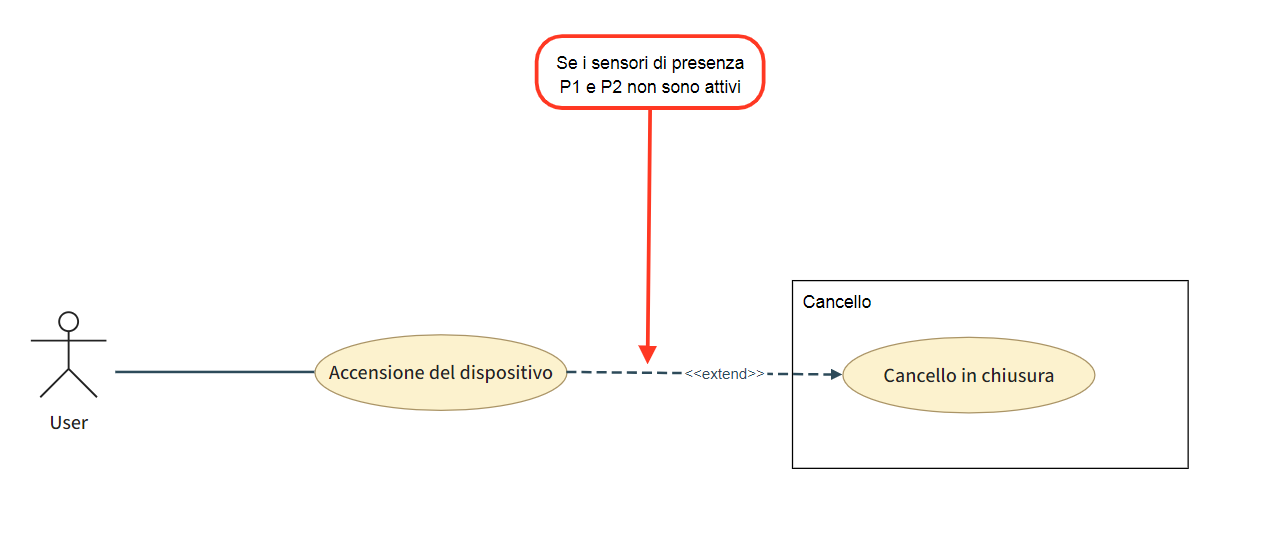
\includegraphics[width=0.9\textwidth]{figures/usecase_9.png}
    \caption{Chiusura Automatica}
    \label{usecase9}
\end{figure}


\section{General Use Case}
\begin{figure}[H]
    \centering
    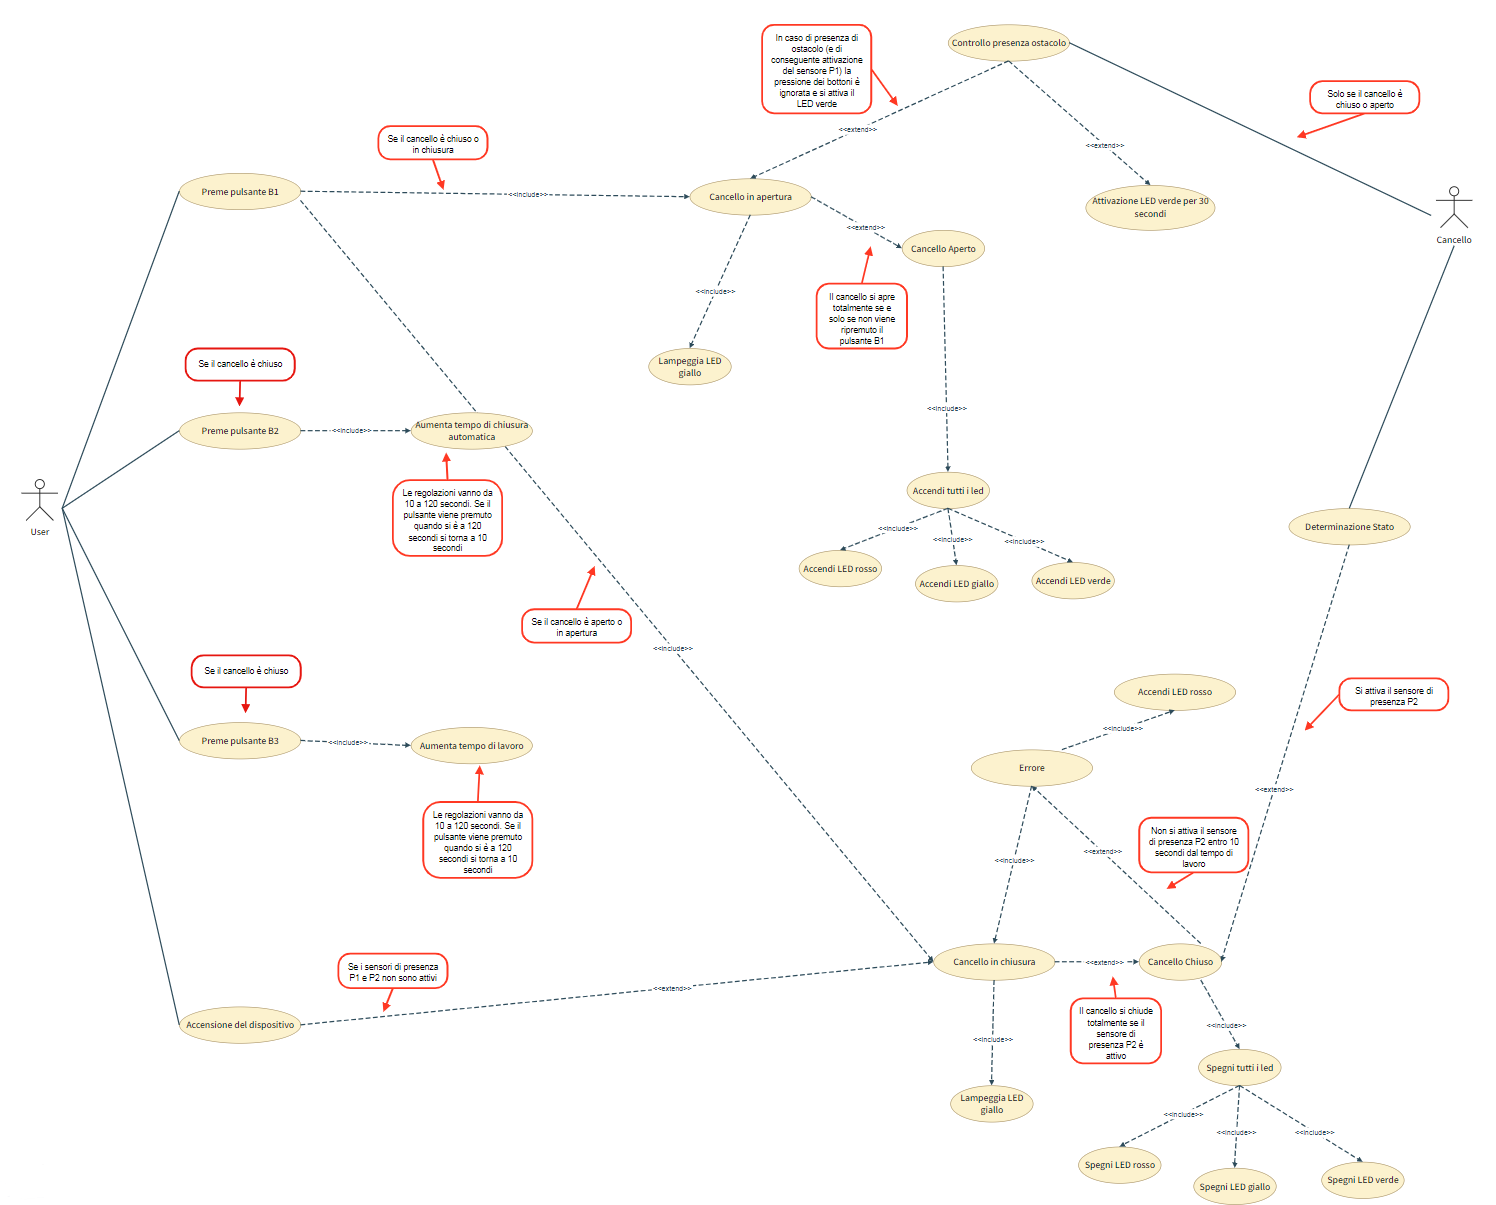
\includegraphics[width=1\linewidth]{figures/generalusecases.png}
    \caption{Use Cases Generale}
    \label{general}
\end{figure}